\documentclass[12pt,oneside]{article}
\usepackage[margin=1in]{geometry}
\usepackage{setspace}
\onehalfspacing
\usepackage{amsmath,amssymb,amsthm}
\usepackage{graphicx}
\usepackage{caption}
\usepackage{subcaption}
\usepackage{booktabs}
\usepackage{float}
\usepackage{hyperref}
\usepackage{cleveref}
\usepackage[table,xcdraw]{xcolor}
\usepackage{natbib}
\usepackage{listings}
\usepackage{array}
\usepackage{enumitem} % Added for itemize options
\usepackage{accents} % Added for \underaccent

% Custom theorem environments
\theoremstyle{definition}
\newtheorem{theorem}{Theorem}[section]
\newtheorem{lemma}[theorem]{Lemma}
\newtheorem{definition}[theorem]{Definition}
\newtheorem{claim}[theorem]{Claim}
\newtheorem{corollary}[theorem]{Corollary}
\theoremstyle{remark}
\newtheorem*{proof*}{Proof}

% Custom commands
\newcommand{\ubar}[1]{\underaccent{\bar}{#1}}
\newcommand{\E}{\mathbb{E}}
\newcommand{\Var}{\mathrm{Var}}

% Table alignment for regression results
\newcolumntype{L}[1]{>{\raggedright\arraybackslash}p{#1}}
\newcolumntype{C}[1]{>{\centering\arraybackslash}p{#1}}
\newcolumntype{R}[1]{>{\raggedleft\arraybackslash}p{#1}}

% Code styling
\lstset{
  basicstyle=\ttfamily\small,
  numbers=left,
  numberstyle=\tiny\color{gray},
  stepnumber=1,
  numbersep=10pt,
  backgroundcolor=\color{lightgray!20},
  keywordstyle=\color{blue},
  commentstyle=\color{green!60!black},
  stringstyle=\color{red!60!black},
  breaklines=true,
  frame=single,
  captionpos=b
}

% Bibliography setup
\bibliographystyle{ecta}

% Title and author
\title{Testing for redatory pricing in airline industry. Welfare effects.}
\author{Nikita Akimov\thanks{Haas School of Business, University of California Berkeley, akimovh@berkeley.edu}}
\date{\today}

\begin{document}

\maketitle

\section{Motivation}

\subsection{Predatory pricing}

Fair market competition is widely regarded by economists as beneficial to economic welfare, and policymakers actively seek to promote and protect it. The Sherman Act explicitly prohibits firms from “monopolizing, or attempting to monopolize… any part of trade or commerce.” Given these legal and economic priorities, it is unsurprising that detecting anticompetitive firm behavior is one of the central topics in industrial organization research. I aim to contribute to that effort by developing a test for one specific form of such behavior: predatory pricing.

Predatory pricing, as defined by \cite{Bolton2000}, refers to a “price reduction that is profitable only due to the increased market power the predator gains by eliminating, disciplining, or otherwise inhibiting the competitive behavior of a rival or potential rival.” The simplest mechanism of predatory pricing unfolds in two distinct phases. During the predation phase, the predator sets prices low enough to drive the target firm's profits into negative territory, forcing its exit or significantly weakening its market position. Once competition diminishes, the recoupment phase follows, during which the predator raises prices sufficiently to recover the losses incurred during the predation phase. This strategy allows the firm to capitalize on its enhanced market power, ultimately undermining fair competition.

\textcolor{red}{Paragraph about not only acedimic interest, but policy too.} 

\subsubsection{Feasibility and rationality}
The arguments presented here are inspired by \cite{Ordover1989}, who discuss predation in detail. The feasibility and profitability of predatory pricing have long been contentious topics of discussion. Critics who challenge its viability typically cite three key objections: the recoupment problem, the high cost of predation, and the critique of asymmetry in financial constraints. The following paragraphs discuss these arguments and the conditions under which they may not hold.

One of the primary objections to the feasibility of predatory pricing is the recoupment problem—the concern that once prices rise during the recoupment phase, new entrants may reappear, and consumers may either switch to substitutes or reduce their demand if prices increase too sharply. However, in markets with high entry barriers, particularly those characterized by significant sunk costs—such as pharmaceuticals, telecommunications, automobile manufacturing, etc.—this risk is less pressing for the predator, as entry occurs infrequently. Moreover, the reputation effect can further discourage competition: if a firm establishes a reputation for aggressively defending its market share, potential entrants may be deterred from challenging it in the future. Finally, the presence of switching costs can further insulate the predator's position by locking in consumers, making the market less attractive for new competitors.

A second major concern regarding the feasibility of predatory pricing is its high cost for the predator and the uncertainty of success. Predatory pricing often requires sustained losses, which may be prohibitively expensive, particularly if competitors withstand the pressure longer than expected. The predator risks depleting its capital before achieving market dominance. Additionally, \cite{McGee1958}’s critique of the Standard Oil case highlights a critical challenge: “the costs of a predatory price-cutting strategy tend to increase with the size of the market share of the predator, whereas the rival's losses are smaller the smaller is its market share.” However, these arguments tend to oversimplify market dynamics. A firm can mitigate the costs of predation through price discrimination across markets or consumer segments, allowing it to maintain higher prices where competition is weak while targeting price cuts where they are most effective in eliminating rivals. This argument has become increasingly compelling with advancements in technology, which have made price discrimination easier to implement. Moreover, even if a firm fails to drive a competitor out of the market, it may still benefit from reputation gains, deterring future challengers. Thus, while predatory pricing is costly and uncertain, strategic implementation can significantly enhance its viability.

The final major critique of predation models is their reliance on the "long purse" or "deep pocket" assumption, which posits that the predator has greater financial resources, allowing it to outlast competitors in a predatory price war. The first point to consider is that, under complete information, predation should not occur in equilibrium—if the prey knows it cannot survive, it will exit the market immediately or choose not to enter in the first place. However, \cite{Benoit1984} demonstrated that when financial constraints are not common knowledge, entry can still occur in equilibrium. If financial asymmetry is assumed, it is necessary to explain the origin of these resource differences. A reasonable question to ask is: why can’t the prey simply borrow enough money to survive the predation phase? \citet{Fudenberg1985, Fudenberg1986} addressed this issue using the theory of financing under asymmetric information. Their argument hinges on the idea that a firm’s ability to borrow depends on its net asset value. If the predator is able to drive the prey’s value below the threshold required for financing, the prey loses access to credit, making survival impossible.

So far, I have discussed the feasibility of predation. But what about its rationality? For a firm to engage in predatory pricing, it must be a long-run utility-maximizing strategy. \cite{McGee1958} argued that merger is always a superior alternative to predation, as a merged firm enjoys higher profits during the predation phase and the same profits as the predator during the recoupment phase. However, several counterarguments challenge this view. First, reputation effects matter—if a firm consistently chooses to merge rather than fight, it may encourage future entry, making predation a more viable strategy in multi-market or multi-entrant contexts. Second, legal constraints can make mergers prohibitively difficult or outright illegal, limiting their practicality as an alternative. Finally, predation itself can serve as a bargaining tool during merger negotiations, allowing the predator to secure more favorable terms by weakening the target firm before acquisition.

In summary, while numerous barriers discourage firms from engaging in predatory pricing, certain market conditions can still make it a viable strategy. \textcolor{red}{Sentence with reference on some work on evidence of predation.} Given this possibility, it is crucial to consider the tools and methods needed to detect predation effectively.



\subsubsection{Testing for predation}



The main challenge in detecting predation is that, unlike collusive behavior, price-cutting is an inherent part of market rivalry. In many industries, firms engage in intense price wars, leading to temporary price reductions that may serve legitimate business purposes—such as responding to a competitor’s discount or clearing out excess inventory. From an external perspective, such pricing strategies can resemble predatory pricing, even when they reflect normal competitive behavior rather than a deliberate strategy to eliminate rivals and recoup losses later.

A common approach to identifying predation is to compare observed prices with specific cost measures. This method was first introduced by \cite{Areeda1975}, who suggested using average variable cost as a proxy for marginal cost. However, a major flaw in this approach is its heavy reliance on accurate cost estimation, which is notoriously difficult. Even when cost data are available, distinguishing between short-run marginal or variable costs and full accounting costs presents additional challenges, making it difficult to determine whether pricing is truly below cost. Later legal standards for proving predation introduced an additional hurdle: demonstrating that the predator would be able to raise prices later. This requirement makes it even more difficult to establish a clear case of predatory pricing in court, as it demands evidence not only of below-cost pricing but also of the firm’s ability to recoup losses through future market power.

To overcome these difficulties, I plan to leverage recent advancements in conduct testing theory, particularly the approache discussed in \cite{Backus2021}. These methods offer a more robust framework for distinguishing predatory pricing from legitimate competition. I detail my approach in the following sections. 

\subsubsection{Welfare effects of predatory pricing}
\textcolor{red}{Write a paragraph about welfare}
\subsection{Airline industry: Southwes vs Hawaiian case}

\subsubsection{Airline industry as an opportunity for predation}

The modern history of airline competition began with the Airline Deregulation Act of 1978, which removed federal control over fares, routes, and market entry. In the aftermath, during the late 1970s and 1980s, fierce competition ensued, leading to intense price wars. Many smaller and poorly managed airlines could not survive, resulting in bankruptcies and industry consolidation. Major mergers followed, gradually forming larger carriers like United, American, and Delta, which became dominant players. These airlines adopted the hub-and-spoke system, a network model in which flights are routed through a central hub airport that connects multiple destinations. They transformed their hubs into “fortresses,” establishing dominance on key routes—often accompanied by fare increases. Starting in the 1990s, low-cost carriers began to grow in popularity. Examples include Southwest, JetBlue, Frontier, and Spirit, which focused on underserved point-to-point markets and offered lower fares than the major airlines. As a result, by the end of the 2010s, almost 90\% of the domestic market was concentrated among eight major carriers.\footnote{Bureau of Transportation Statistics: \href{https://www.transtats.bts.gov/}{https://www.transtats.bts.gov/}} The Covid-19 pandemic severely impacted the airline industry, especially low-cost carriers, due to travel restrictions and reduced demand. However, in the long run, the overall market structure—major players and competition levels—remained relatively stable.

The airline industry faces significant entry barriers. To begin with, the sunk costs of buying or leasing aircraft require massive upfront investments. On top of that, aircraft manufacturers typically have backlogs of 2 to 5 years, delaying the payoff and demanding substantial early capital. Furthermore, economies of scale give established airlines a significant advantage, making it difficult for new entrants to compete on costs like fuel, maintenance, and labor. Airport capacity is limited, with most slots already controlled by existing airlines, leaving new entrants struggling to gain access. Compounding these challenges, the industry is heavily regulated by the government, and complying with these regulations requires considerable time and investment. As a result, these factors not only make the emergence of new airlines nearly impossible, but also hinder existing airlines from entering well-served routes or key airports. For example, American and Delta have dominant positions at JFK, controlling most lucrative international routes and domestic slots. Consequently, this forced United to choose Newark as its hub for the New York metro area, despite Newark’s less convenient location for Manhattan-bound travelers compared to JFK or LaGuardia.

Another widely adopted strategy in the airline industry is loyalty programs and co-branded credit cards. Multiple studies have demonstrated that these programs create significant switching costs for consumers.\footnote{\textcolor{red}{add references}} When discussing the airline industry, it is impossible to avoid the topic of price discrimination. Price dispersion within the same route-carrier pair largely depends on the level of market competition, \textcolor{red}{add references}. Additionally, it is important to highlight the widespread practice of dynamic pricing, where ticket prices fluctuate based on demand, booking time, and other market conditions.

All of the above makes the airline industry particularly attractive for study, especially for empirical work. I will examine the main findings in the literature in the Literature Review section. At the same time, these factors support my assumption regarding the feasibility and attractiveness of predatory pricing in the airline industry.



\subsubsection{Southwest vs Hawaiian.}

The Hawaiian airline market is distinct from other domestic U.S. markets due to its geographical isolation, reliance on air travel for both inter-island and mainland connectivity, and a tourism-driven demand structure. Like all domestic markets, the Hawaiian market faced fierce competition following the Airline Deregulation Act of 1978. However, due to its unique conditions, this competition had a more localized effect. In 2008, Aloha Airlines liquidated under Chapter 7 bankruptcy, seemingly leaving Hawaiian Airlines as only major player there. While larger carriers offered flights between Hawaii and the mainland, along with international routes across the Pacific, Hawaiian Airlines faced virtually no competition in the inter-island market, which accounted for almost 40\% of the total Hawaiian market. Starting the 2017 Hawaiian Airlines became a monopoly in inter-island flights and substantially raised prices. The airline relied heavily on the inter-island segment, with more than 60\% of its passenger flow being interstate. This strategy proved successful, as Hawaiian Airlines reported an average annual profit of XXX million dollars between 2010 and 2018.
 
Everything changed when Southwest entered the Hawaiian market in 2019 as part of its broader expansion in the late 2010s. The aggressiveness with which Southwest enters new markets is well-known in the industry and has even earned its own name—the “Southwest effect.” Southwest itself wasn’t shy about displaying its extra-competitive nature: in early 2021, a photo of wall art at Southwest’s ETOPS center at Oakland Airport depicting a shark eating its rivarlies leaked onto the internet.
\begin{figure}[H]
  \centering
  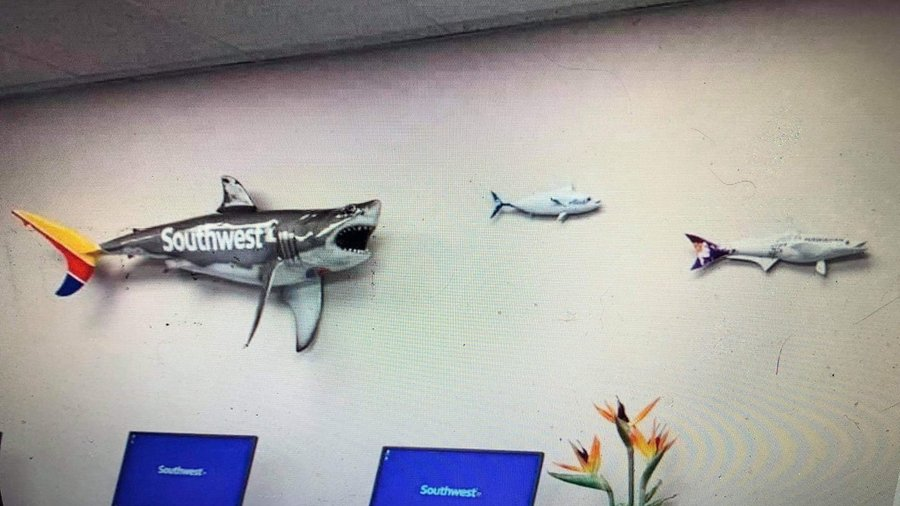
\includegraphics[scale=0.5]{plots_and_pictures/southwest-shark_900x506x1440-810-0-135.jpg}
  \caption{Wall art in Southwest ETOPS center at Oakland Airport}
\end{figure}
 Moreover, Capt. Jon Weaks, head of the union representing Southwest’s pilots, once described their expansion strategy as “predatory and opportunistic—which we like.”\footnote{\href{https://www.wsj.com/articles/southwest-airlines-covid-expansion-airports-11605296205}{https://www.wsj.com/articles/southwest-airlines-covid-expansion-airports-11605296205}} Southwest’s fares were substantially lower than Hawaiian’s.\textcolor{red}{(Insert info on percentage difference here.)}
 
 Note the fact, that it is a common practice for companies to penetrate a new market with lower prices to attract a share of a rival’s customer base. However, usually they are last for a really short time, In our case even in 2022–2023, when the domestic airline industry had fully recovered after pandemic and Southwest had been operating in Hawaii for more than three years, it continued offering extremely low fares for inter-island flights. This raised questions about a potential predatory strategy. During an internal earnings call, Hawaiian Airlines executives noted that Southwest’s fares were unsustainably low and operating at a loss.\footnote{\textcolor{red}{link here}} Even Southwest’s own investors expressed concerns that these prices were 'clearly unsustainable'.\footnote{\textcolor{red}{Link to Southwest financial call}}

 Fierce competition from Southwest on Hawaiian Airlines’ biggest routes, combined with the pandemic crisis and the wildfires in Maui, resulted in a sharp decline in Hawaiian’s profits. The airline posted net losses in 14 of the past 15 quarters. As a result, in a bid for survival, Hawaiian Airlines was acquired by Alaska Airlines at the end of 2023. Alaska paid \$1.9 billion, including \$900 million in Hawaiian Airlines’ debt. This acquisition further consolidated an already highly concentrated market. Right after the acquisition announcement, inter-island flight prices rose, and \textcolor{red}{sometime later}, Southwest adjusted its Hawaiian strategy.

 I believe that Southwest’s strategy was to induce Hawaiian Airlines to exit the market and become a monopolist on inter-island flights, but they miscalculated the resistance with which the local carrier fought back. Several factors support this theory. First, Southwest does not have a hub in Hawaii; its crew flies in from the mainland daily, which should be expensive, suggesting that its marginal costs are quite high. Second, publicly available information—including Southwest’s press releases, leaked photos, observed pricing behavior, and less aggressive competition after the acquisition announcement—all align with this hypothesis. Third, external organizations and experts have accused Southwest of engaging in predatory pricing.\footnote{\textcolor{red}{American Economics Liberties Report}} Additionally, the incentive for such behavior is clear: controlling inter-island flights would create even higher barriers for competitors and allow Southwest to establish dominant power on mainland-Hawaii routes. Southwest’s fares were among the lowest in the domestic market, further supporting this view. Finally, even Southwest’s own activist investor, Elliott Management, reportedly considered this strategy unsuccessful.


\section{Literature Review}

\textcolor{red}{TBD}

This paper contributes to three main strands of economic literature. First, it adds to the research on predatory pricing, a topic that has received relatively limited attention in the context of IO empirical work. Second, it enriches the broader empirical literature on competition in the airline industry by examining pricing strategies following market entry. Third, it contributes to the field of conduct testing in structural models by applying recent methodological advancements to the study of predatory pricing.


This paper relates to broad literature on predatory pricing models. The models based on asymmetric financial constrains (the long purse) might be seen in Telser(1966), Benoit (1984), Fudenberg and Tirole (1986b). Models based on signaling can be found in ... Reputation models of predation might be seen in:. Other filed of theoretical works is a modeles od predation in presence of learning by doig, a great examples of such work are ....


Empirical investigations of predatory pricing based on market data remain scarce. Early descriptive work in this area can be traced back to McGee (1958) and Elzinga (1970), both of whom examined historical data and found little evidence of predatory behavior. Burns (1986) explored the effects of price cuts on acquisition costs, while more recent contributions include Genesove and Mullin (2006), who leveraged advancements in industrial organization theory to establish a competitive price lower bound as a benchmark for identifying predation. However, much of this research relies on relatively old data, often from the early 20th century, and focuses primarily on homogeneous markets.

Our study advances this literature in several important ways. To our knowledge, it represents the first attempt to test for predatory pricing using modern market data in an environment characterized by product differentiation. Furthermore, we propose a more robust approach to identifying predatory pricing, drawing on recent developments in conduct testing theory. By directly comparing equilibrium models, our methodology not only allows for the detection of predatory pricing but also sheds light on the underlying mechanisms driving such behavior.

The airline industry has been extensively studied, particularly in the context of demand and supply modeling. Foundational work in this area includes Berry et al. (1996), Berry and Jia (2010), Ciliberto and Williams (2014), Peters (2006), Israel et al. (2013), and Das (2019), all of whom developed structural models to analyze competition, pricing, and market structure. More closely related to our study is Busse (2002), who examined the relationship between a carrier’s financial position and the likelihood of initiating a price war. Another key contribution is Goolsbee and Syverson (2008), who investigated how incumbents respond to the threat of entry, demonstrating that airlines significantly lower fares when facing potential competition from Southwest Airlines. Our work contributes to this strand of literature by focusing explicitly on price wars following market entry, providing new insights into post-entry competitive dynamics.

A third body of research relevant to our study involves conduct testing in structural models of demand and supply. The foundational work in this domain includes Bresnahan (1982), who introduced the concept of 'demand rotations' as a tool for identifying firm conduct. More recent advancements in the field include contributions by Nevo (2021), Berry et al. (2014), Pakes (2017), and Backus et al. (2021), all of whom developed methodologies to test for firm collusion and pricing above competitive levels. In contrast to this existing work, our study extends these methodological frameworks to examine predatory pricing, thereby broadening the scope of conduct testing applications in industrial organization.

In summary, our research builds upon and extends three key areas of economic literature: empirical studies of predatory pricing, competition in the airline industry, and conduct testing in structural models. By integrating modern market data and employing advanced empirical techniques, our study offers new insights into the strategic use of pricing as a competitive tool, with implications for both policy and economic theory.

\section{Formal Model (i.e., with math)}


\subsection{Demand Side}
A standard logit utility for consumer $i$ choosing product $j$ in period $t$ is given by
\begin{equation}
U_{i,j,t} 
= - \alpha p_{jt} + X_{jt}'\beta + \varepsilon_{jt} + \epsilon_{ijt},
\end{equation}
where
\begin{itemize}[leftmargin=2em]
    \item $p_{jt}$ is the price of product $j$ in period $t$,
    \item $\alpha > 0$ is the (common) price sensitivity parameter,
    \item $X_{jt}$ are observed (time-varying) product characteristics,
    \item $\varepsilon_{jt}$ are unobserved product-specific demand shock at period $t$,
    \item $\epsilon_{ijt}$ is unobserved product and consumer-specific demand shock at period $t$, which has an i.i.d. Type I Extreme Value error.
\end{itemize}








\subsection{Supply side: Predation model}
Consider two products: a "local small firm" (L) and a "predator" (P). And consider three-phase model.

\begin{itemize}[leftmargin=2em]
    \item In Phase 1, only the local small firm is active (monopoly).
    \item In Phase 2, both the local firm and the predator are active.
    \item In Phase 3, only the predator is active (after the local firm exits).
\end{itemize}

\subsubsection{Phase 1 (Monopoly by Local Small Firm)}
The local small firm (L) is the sole producer, charging its monopoly price $p_{L}^{M}$ until the predator arrives. We can write the local firm's profit in Phase 1 as:
\begin{equation}
\pi_{L,1}(p_L^M) = (p_L^M - c_L) \cdot Q_L(p_L^M),
\end{equation}
where $c_L$ is the (constant) marginal cost of the local firm, and $Q_L(\cdot)$ is the local firm's demand under the logit specification.

\subsubsection{Phase 2 (Predatory Pricing)}
Let $T$ be the maximum number of periods the predator is willing or able to price ``aggressively''. Predator knows $T$, however for small firm it is a random variable governed by some distribution that the local firm does not know, but updates beliefs about via Bayes' rule.
During these $T$ periods, the predator \emph{may} choose to set a ``low'' (possibly below-cost) price in order to drive out the local firm. After $T$ periods (if the local firm is still in the market), the predator reverts to a higher, more ``normal'' or ``competitive'' price. 
Both the ``predatory'' price and the ``competitive'' price will emerge as solutions of the predator's \emph{static or dynamic} pricing problems.

\section{Predator's Dynamic Optimization}

\subsection{Defining Two Benchmark Prices Endogenously}

\begin{enumerate}
\item \textbf{$p_{Pt}^{\text{comp}}$ (competitive or normal price).} 
If the predator is \emph{not} trying to induce exit (or if no exit is possible), it solves a \emph{static} best-response (or monopoly) problem each period. Formally, in a single-period setting against the local firm's price $p_{Lt}$, the predator chooses
\[
p_{Pt}^{\text{comp}}
\;=\;
\arg\max_{p_P}
\Bigl\{\,
\bigl(p_P - c_P\bigr)\,
Q_P\bigl(p_P,\;p_{Lt}\bigr)
\Bigr\},
\]
i.e.\ the usual Bertrand best-response (or monopoly price if the local firm is not active).

\item \textbf{$p_{Pt}^{\text{pred}}$ (predatory price).}
If the predator \emph{is} trying to induce exit---trading off short-run losses against a \emph{future} gain of monopoly---then in a \emph{dynamic} sense, it chooses
\[
p_{Pt}^{\text{pred}}
\;=\;
\arg\max_{p_P}
\Bigl\{
(p_P - c_P)\,Q_P\bigl(p_P,\,p_{Lt}\bigr)
\;+\;
\delta \;\mathbb{E}\!\bigl[V_P^{\text{next}}(\text{state after choosing }p_P)\bigr]
\Bigr\},
\]
where $V_P^{\text{next}}$ is the continuation value if the predator charges $p_P$ this period (potentially raising the probability that the local firm exits). 

\end{enumerate}

\noindent
In equilibrium, the predator compares the expected net present value (NPV) from charging the predatory price \emph{versus} the NPV from charging the competitive price. Whichever price yields a higher expected payoff---accounting for the possibility of local firm exit---is chosen in that period.

Hence, from a \emph{single-period perspective}, you may see the predator ``pick from two extremes,'' but behind the scenes, \emph{both} $p_{Pt}^{\text{pred}}$ and $p_{Pt}^{\text{comp}}$ emerge from \emph{optimization problems}---they are not exogenous.

\subsection{A Simple Finite-Horizon Formulation with Known $T$}

To make this concrete, suppose:
\begin{enumerate}
\item The predator has at most $T$ periods in which it can or wants to engage in ``predatory'' pricing.
\item After $T$ periods (if the local firm is still active), the predator \emph{must} charge the competitive price from then on (earning duopoly profits).
\item If the local firm \emph{exits earlier} (say at $\tau < T$), the predator obtains \emph{monopoly} profits from $\tau$ onward.
\end{enumerate}

\noindent
Let
\[
\tau \;=\;
\text{(random) time the local firm exits},\quad
1 \;\le\; \tau \;\le\; T\quad
\text{or}\quad \tau=\infty \text{ if it never exits}.
\]
Let $\delta \in (0,1)$ be the discount factor.

\subsubsection{Predator's Value Function}

Define the \emph{state} each period as
\[
\text{State}_t \;=\;
\Bigl(\,\text{whether L is in/out},\;
\text{how many predation periods remain},\;
\text{L's beliefs},\;\ldots \Bigr).
\]

\noindent
For $k \in \{0,1,\dots,T\}$, let
\[
V_P\bigl(\text{L in},\, k\bigr)
\;=\;
\text{maximum discounted payoff to the predator when the local firm is active and there are $k$ ``predation periods'' left.}
\]
\begin{itemize}
\item If $k=0$, the predator can no longer (or chooses not to) do predation, so it simply charges $p_{Pt}^{\text{comp}}$ (the static best-response) thereafter.
\item If $k>0$, the predator \emph{can} choose a low price (possibly below cost).
\end{itemize}

\noindent
\textbf{Case (i): Local firm in, $k>0$.}
\[
V_P(\text{L in},\, k)
\;=\;
\max_{p_P}
\Bigl\{
\bigl(p_P - c_P\bigr)\,Q_P\bigl(p_P,\;p_{L}^*(p_P)\bigr)
\;+\;
\delta \;\mathbb{E}\Bigl[
V_P\bigl(\text{L in/out next},\;k_{\text{next}}\bigr)
\Bigr]
\Bigr\}.
\]
Here:
\begin{itemize}
\item ``$\text{L in/out next}$'' depends on whether the local firm decides to stay or exit.
\item ``$k_{\text{next}}$'' becomes $(k-1)$ if the predator is using one of its $k$ ``predation moves.'' It might remain $k$ if the chosen price is effectively the normal best-response.
\end{itemize}

\noindent
In practice, the predator might \emph{solve for two candidate prices}---the ``predatory price'' $p_{P}^{\text{pred}}(k)$ and the ``competitive price'' $p_{P}^{\text{comp}}$---and then choose whichever yields the higher payoff. Symbolically:
\[
\begin{aligned}
p_{P}^{\text{pred}}(k)
&=\arg\max_{p}
\Bigl\{\,
(p - c_P)\,Q_P(p,\dots)
\;+\;
\delta\,\mathbb{E}\bigl[V_P(\dots,k-1)\bigr]
\Bigr\},\\[6pt]
p_{P}^{\text{comp}}
&=\arg\max_{p}
\Bigl\{\,
(p - c_P)\,Q_P(p,\dots)
\Bigr\}.
\end{aligned}
\]
Then
\[
V_P(\text{L in},\, k)
\;=\;
\max
\Bigl\{
\bigl[(p_{P}^{\text{pred}}(k) - c_P)\,Q_P(\dots)
+ \delta\,\mathbb{E}\bigl[V_P(\dots,k-1)\bigr]\bigr],
\;\;
\bigl[(p_{P}^{\text{comp}} - c_P)\,Q_P(\dots)
+ \delta\,\mathbb{E}\bigl[V_P(\dots,k)\bigr]\bigr]
\Bigr\}.
\]
\emph{If the ``predation strategy'' is chosen, you move to $(k-1)$ predation periods left. If the ``competitive'' price is chosen, you remain at $k$.}

\vspace{1em}
\noindent
\textbf{Case (ii): Local firm out.}
If the local firm has exited, the predator obtains \emph{monopoly} profits forever:
\[
V_P(\text{L out})
\;=\;
\sum_{s=0}^{\infty}
\delta^{\,s}
\bigl[
(p_{P}^{M} - c_P)\,Q_{P}(p_{P}^{M})
\bigr],
\]
where $p_{P}^{M}$ is the predator's static monopoly price (only the outside good is present to compete).

\vspace{1em}
\noindent
\textbf{Case (iii): $k=0$ and local firm in.}
Then the predator does normal/competitive pricing:
\[
V_P(\text{L in},\, 0)
\;=\;
\max_{p_P}
\Bigl\{
(p_P - c_P)\,Q_P\bigl(p_P,\dots\bigr)
\;+\;
\delta\,\mathbb{E}\bigl[V_P(\dots,\, 0)\bigr]
\Bigr\}.
\]
That is, with no more low-price moves available, the predator reverts to a standard repeated duopoly pricing problem.

\subsection{The Local Firm's Exit Decision and Belief Updating}

Meanwhile, the local firm each period decides whether to stay or exit, based on
\[
V_L(\text{stay};\,k)
\;=\;
\max_{p_L}
\Bigl\{
\pi_L\bigl(p_L,\,p_P(k)\bigr)
\;+\;
\delta\,\mathbb{E}\bigl[V_L(\dots,\,k')\bigr]
\Bigr\}
\quad\text{versus}\quad
V_L(\text{exit}) \;=\; 0.
\]
Here:
\begin{itemize}
\item $p_{P}(k)$ is the predator's equilibrium price if it has $k$ predation moves remaining.
\item If the local firm forms beliefs that $k$ might be large, it knows the predator might keep price low for many periods, reducing its expected future profit.
\item Each period, observing the predator's actual price (low or high) updates the local firm's posterior on $k$ (or on the distribution of $T$).
\end{itemize}
If \emph{staying} yields negative expected NPV (given updated beliefs and continuing low prices), the local firm exits.

\section{Final (Refined) Predator's Problem Equation}

Putting it all together, in each state $(\text{L in}, k)$, the predator solves a dynamic program:
\[
\boxed{
V_{P}(\text{L in},\, k)
\;=\;
\max_{\,p_{Pt}\,\in\,\mathcal{P}}
\Bigl\{
\bigl(p_{Pt} - c_{P}\bigr)\,Q_{P}\bigl(p_{Pt},\,p_{L}^{*}(p_{Pt})\bigr)
\;+\;
\delta\;\mathbb{E}\bigl[
V_{P}\!\bigl(\text{L in/out next},\,k_{\text{next}}\bigr)
\bigr]
\Bigr\}.
}
\]

\begin{itemize}
\item $\mathcal{P}$ is the feasible set of prices (possibly including below-cost prices).
\item If $p_{Pt}$ is ``low enough,'' we say the predator uses one period of predation, so next state has $(k-1)$ moves left.
\item If $p_{Pt}$ is effectively ``competitive,'' then next state is still $k$ moves left.
\item ``L in/out next'' is determined by the local firm's best-response decision and beliefs.
\end{itemize}

\noindent
Thus, in equilibrium you \emph{end up} with two candidate solutions each period:
\begin{enumerate}
\item \emph{Predatory price} $p_{Pt}^{\text{pred}}(k)$ = the solution when the predator is actively trying to accelerate L's exit.
\item \emph{Competitive price} $p_{Pt}^{\text{comp}}$ = the static best-response price if the predator is not trying to induce exit (or if it has no remaining predation moves).
\end{enumerate}

\noindent
The predator picks whichever yields the higher payoff in that state. In other words, ``predatory'' and ``competitive'' prices are both found by optimization but reflect different strategic aims (exit-inducement vs.\ normal pricing).

\section{Takeaways}

\begin{itemize}
\item \textbf{Endogenous Predatory vs.\ Competitive Price.}\\
You do \emph{not} have to treat $p_{Pt}^{\text{pred}}$ or $p_{Pt}^{\text{comp}}$ as exogenous or ``pre-determined.'' In the dynamic game, the predator \emph{optimizes} across \emph{all feasible prices} each period, balancing short-run and long-run payoffs.

\item \textbf{Length of Predation $T$.}\\
If $T$ is \emph{known} and finite, you can implement backward induction (or dynamic programming) to solve for the predator's value function and optimal policy. If $T$ is \emph{unknown} to the local firm, it updates beliefs each period based on whether the predator continues to charge a low price.

\item \textbf{Equilibrium.}\\
The local firm's stay/exit decision is optimal given its beliefs. The predator's low price is optimal given the local firm's likely response and the finite or stochastic number of predation periods. This yields a Bayesian Perfect Equilibrium (or Markov-Perfect Equilibrium if you treat beliefs as part of the state).
\end{itemize}
\paragraph{Phase 3: Predator as Monopolist}

If L exits at time $t$, then from $t+1$ onward, P is the only firm:
\[
p_{Pt}^M
\;=\;
\arg\max_{p_P}\;\bigl(p_P-c_P\bigr)\,Q_P(p_P).
\]
Phase 3 yields monopoly profits for P indefinitely (or until some terminal horizon).

\section{3. Parameters to Estimate}

\begin{enumerate}
%   \item \textbf{Demand parameters}: $\{\alpha,\bm{\beta}\}$, possibly distribution parameters for $\xi_{jt}$.
  \item \textbf{Cost parameters}: $\{c_L,\,c_P\}$ if not taken as given.
  \item \textbf{Dynamic/game parameters}:
  \begin{itemize}
    \item $\delta$: discount factor.
    \item Distribution of predation phase length (e.g.\ parameter $\gamma$ of a geometric distribution).
    \item Priors $\pi_0(\theta)$ that govern the local firm's belief updating.
  \end{itemize}
  \item \textbf{Strategy function parameters}: If $p_{Pt}^{\text{pred}}$ and $p_{Pt}^{\text{comp}}$ are fixed, no additional estimation is needed for these. Otherwise, specify their functional form.
\end{enumerate}

\section{4. Identification}

\begin{itemize}
  \item \textbf{Demand side}: Standard logit identification requires exogenous variation in prices or valid instruments.
  \item \textbf{Costs}: If $c_L,c_P$ are truly known, no further identification needed. Otherwise, cost data or supply-side variation is required.
  \item \textbf{Dynamic parameters}: The time-series of observed (predatory vs.\ competitive) prices, together with the local firm's observed exit decisions, identifies the distribution of predation length and the discount factor (or at least constrains it).
  \item \textbf{Belief updating}: Observing how quickly L exits (conditional on sequences of predatory prices) identifies L's beliefs about predation length.
\end{itemize}

\section{5. Equilibrium Conditions}

We look for a (Markov-Perfect or Bayesian) equilibrium where:
\begin{enumerate}
  \item \textbf{Predator's pricing strategy}:
  \[
  p_{Pt}^*
  \;=\;\arg\max_{p_{Pt}\in\{p_{Pt}^{\text{pred}},\,p_{Pt}^{\text{comp}}\}}
  \Bigl\{
  \pi_{Pt}(p_{Pt},p_{Lt}^*,\text{State}_t)
  +\delta\,\mathbb{E}\bigl[V_P^{t+1}(\text{State}_{t+1})\bigr]
  \Bigr\}.
  \]
  \item \textbf{Local firm's stay/exit and price decision}:
  \[
  \bigl(\text{Stay}_t^*,\,p_{Lt}^*\bigr)
  \in
  \arg\max_{\substack{\text{Stay}_t \in\{0,1\}\\p_{Lt}}}
  \Bigl\{
    \text{Stay}_t\,\bigl[\pi_{Lt}(p_{Lt},p_{Pt}^*,\text{State}_t)
    +\delta\,\mathbb{E}[V_L^{t+1}(\text{State}_{t+1})]\bigr]
  \Bigr\}.
  \]
  \item \textbf{Bayes updating} for L's beliefs:
  \[
  \pi_{t+1}(\theta)
  \;=\;
  \frac{\Pr(\text{Predator's observed action at }t \mid \theta)\,
  \pi_t(\theta)}{
  \sum_{\theta'} \Pr(\text{Predator's action at }t \mid \theta')\,
  \pi_t(\theta')}.
  \]
  \item \textbf{Consistency}: L's beliefs about P's strategy must match the strategy P actually uses in equilibrium.
\end{enumerate}

\section{6. Potential Moments for Estimation}

To estimate the model, you can use the following data-driven approaches:

\begin{itemize}
  \item \textbf{Demand estimation moments}: Standard logit GMM / MLE (e.g.\ match observed market shares $s_{jt}$ to prices $p_{jt}$ and characteristics $X_{jt}$).
  \item \textbf{Price-setting / dynamic moments}:
  \begin{itemize}
    \item Frequency of predatory vs.\ competitive pricing.
    \item Timing of the local firm's exit.
    \item Duration (number of periods) of low-price episodes before L exits.
  \end{itemize}
  \item \textbf{Structural likelihood}: Write down the probability of each observed path $(p_{Lt},\,p_{Pt},\,\text{exit/stay})$ under the model. Perform maximum likelihood or simulation-based estimation.
  \item \textbf{Method of Simulated Moments (MSM)}:
  \begin{enumerate}
    \item For candidate parameter values, simulate the model many times.
    \item Compute summary statistics (e.g.\ average duration of predation, fraction of markets where L exits, average exit time).
    \item Match these (via minimum distance) to the corresponding empirical statistics.
  \end{enumerate}
\end{itemize}

\section*{Conclusion}

This three-phase model links a standard logit demand system to a dynamic predatory-pricing game with incomplete information about the duration of predation. The key ingredients are:
\begin{itemize}
  \item Demand estimation (logit).
  \item Dynamic game in Phase 2 (predatory vs.\ competitive prices, stay vs.\ exit).
  \item Bayesian updating of the local firm's beliefs about the predator's strategy.
\end{itemize}
Phase 3 arises if and when the local firm exits, yielding a monopoly for the predator. Taking this model to data involves estimating the demand side, costs, and dynamic parameters through observation of actual price paths, exit decisions, and durations of predation.


\section{Data Sources}
\begin{itemize}
    \item What data would you use to pursue your research?
    \begin{itemize}
        \item TBD
    \end{itemize}
    \item How would you collect it? Are there confidentiality issues?
    \begin{itemize}
        \item TBD
    \end{itemize}
    \item What are the limitations of the data?
    \begin{itemize}
        \item TBD
    \end{itemize}
\end{itemize}

\section{Implementation}
\begin{itemize}
    \item What are the two or three "first cut" empirical facts you would look for as evidence of your hypothesis?
    \begin{itemize}
        \item TBD
    \end{itemize}
    \item What methodological challenges would be involved in estimation?
    \begin{itemize}
        \item TBD
    \end{itemize}
\end{itemize}

\section{References}
\bibliography{export}

\end{document}